\documentclass[11pt,a4paper]{article}

% Essential packages
\usepackage[utf8]{inputenc}
\usepackage[margin=1.0in]{geometry}
\usepackage{amsmath,amssymb,amsfonts,amsthm}
\usepackage{booktabs}
\usepackage{graphicx}
\usepackage{subcaption}
\usepackage{hyperref}
\usepackage{natbib}
\usepackage{microtype}
\usepackage{xcolor}
\usepackage{array}
\usepackage{tabularx}
\usepackage{float}

% Hyperref setup
\hypersetup{
    colorlinks=true,
    linkcolor=blue!70!black,
    citecolor=blue!70!black,
    urlcolor=blue!70!black
}

\title{\textbf{Candidate Order Instability in Non-Autoregressive\\Multi-Candidate Transformers}}

\author{
  \textbf{Anshul Saxena} \\
  \texttt{f20221041@hyderabad.bits-pilani.ac.in} \\
  \url{https://github.com/anshull-saxena/candidate-order-instability} \\
  \small{Zenodo DOI: \href{https://doi.org/10.5281/zenodo.22906245}{10.5281/zenodo.22906245}}
}

\date{September 2026}

\begin{document}

\maketitle

\begin{abstract}
Non-autoregressive multi-candidate transformers evaluate classification choices by concatenating candidate-specific marker tokens into a single prompt sequence processed by a bidirectional encoder. Mathematically, a set of candidate classes represents an unordered collection, and an idealized decision rule should exhibit permutation invariance. In this study, we investigate whether candidate presentation order acts as a hidden nuisance variable in such architectures. Evaluating a production-style bidirectional encoder (\texttt{convaiinnovations/laya}) on the Banking77 benchmark across strictly nested candidate subsets ($K \in \{5, 10, 20, 40, 77\}$), we observe that pairwise argmax decision instability ($\mathrm{FR}_{\mathrm{top1}}$) strongly increases with candidate cardinality, rising from $5.70\%$ [3.1\%, 8.4\%] at $K=5$ to $47.28\%$ [42.8\%, 51.9\%] at $K=77$ across random permutations of identical candidate sets. Cross-permutation candidate logit variance expands by $7.5\times$ ($8.40 \to 63.34$). While canonical alphabetical sorting eliminates run-to-run variance by deterministically fixing the serialization string, evaluating against counterfactual reverse-alphabetical sorting ($Z \to A$) induces a $55.83\%$ [47.5\%, 65.0\%] disagreement rate at $K=77$, demonstrating that canonicalization conceals rather than eliminates positional exposure bias. We evaluate inference-time order marginalization over $M$ permutations without architectural retraining: random marginalization monotonically decreases residual decision flip rate to $25.83\%$ [20.3\%, 32.0\%] at $M=5$ while improving calibration (Expected Calibration Error drops from $0.3857$ to $0.0960$), and orthogonal cyclic permutation shifts achieve a residual flip rate of $16.11\%$ [11.9\%, 20.6\%] at equal computational budget. Across 45 pre-specified paired comparisons against native ordering under Benjamini-Hochberg False Discovery Rate control ($q=0.05$), exactly one comparison achieved statistical significance: cyclic shifts ($M=5$) at $K=40$ ($+9.17$ percentage points, unadjusted $p=0.00098$, adjusted $p=0.04395$). At $K=77$, accuracy gains fail FDR significance due to query-level binary outcome variance. Finally, we report a negative replication result: an exploratory $65.0\%$ accuracy finding for cyclic shifts at $K=77$ was an artifact of small-sample unstratified evaluation ($N=40, S=1$) and regressed to $48.06\%$ [39.7\%, 55.6\%] under pre-specified multi-seed replication ($N=120, S=3$). All code, raw data, and statistical verification suites are openly available.
\end{abstract}

\section{Introduction}

In classification, dialogue state tracking, intent routing, and tool selection, a classifier is presented with an input query $q$ and a candidate set $\mathcal{C} = \{c_1, \dots, c_K\}$. In mathematical formulations of classification, $\mathcal{C}$ is an unordered set: the set of choices available to the decision rule does not possess an intrinsic sequence. Consequently, an ideal decision function $f(q, \mathcal{C})$ should be permutation-invariant: for any permutation $\pi \in \mathcal{S}_K$, reordering the candidates prior to presentation should yield identical classifications:
\begin{equation}
f(q, \pi(\mathcal{C})) = f(q, \mathcal{C}).
\end{equation}

In practice, modern transformer-based classifiers often serialize choices into text. In autoregressive language models, choices are presented as prompt lists (e.g., ``Options: (A) ... (B) ...''), which have been repeatedly shown to induce recency or primacy biases \citep{guo2017calibration}. To achieve low-latency inference in agentic routing and intent classification, non-autoregressive multi-candidate transformers \citep{laya2024} evaluate all $K$ candidates simultaneously within a single bidirectional forward pass. In this architecture, candidate strings are concatenated into a single input sequence separated by candidate-specific marker tokens. The sequence is processed by a bidirectional encoder (e.g., RoBERTa; \citealp{liu2019roberta}), and per-candidate classification logits are extracted by projecting the contextualized marker embeddings through a linear head.

While computationally efficient ($O(1)$ forward passes with respect to $K$), serializing unordered choices into a 1D sequence injects artificial positional relationships. Because full bidirectional self-attention couples every token with all other tokens, the contextualized representation of candidate marker $M_k$ is influenced by its absolute position, its relative distance from query tokens, and the semantic identities of its immediate sequence neighbors.

This empirical investigation addresses the question: \textit{Does candidate presentation order act as a hidden nuisance variable in non-autoregressive multi-candidate transformer decision architectures, and how does this sensitivity scale with candidate cardinality $K$?}

To answer this question rigorously, we perform a controlled empirical study using the Banking77 benchmark \citep{casanueva2020efficient} on the open-source \texttt{convaiinnovations/laya} model checkpoint. Our experimental contributions and findings are scoped as follows:
\begin{enumerate}
    \item \textbf{Controlled Distractor Nesting Protocol:} We design a strictly nested candidate-subsampling protocol ($K_5 \subset K_{10} \subset K_{20} \subset K_{40} \subset K_{77}$) over $N=120$ test queries stratified across all 77 intent classes, ensuring that cardinality comparisons are not confounded by stochastic distractor sampling.
    \item \textbf{Order Sensitivity Scaling:} Holding query and candidate sets fixed, random permutations induce an argmax decision flip rate ($\mathrm{FR}_{\mathrm{top1}}$) that increases from $5.70\%$ [3.1\%, 8.4\%] at $K=5$ to $47.28\%$ [42.8\%, 51.9\%] at $K=77$. Cross-permutation candidate logit variance expands by $7.5\times$ ($8.40 \to 63.34$).
    \item \textbf{The Canonicalization Fallacy:} Canonical alphabetical sorting eliminates run-to-run prediction variance ($\mathrm{FR}_{\mathrm{top1}} \equiv 0.0\%$), but counterfactual reverse-alphabetical sorting ($Z \to A$) induces a $55.83\%$ [47.5\%, 65.0\%] disagreement rate at $K=77$. Deterministic serialization locks in exposure bias rather than removing order sensitivity.
    \item \textbf{Inference-Time Order Marginalization:} Without modifying model weights, averaging probability vectors over $M \in \{1, 2, 3, 5\}$ permutations reduces residual decision instability. At $K=77$, random marginalization suppresses residual flip rate to $25.83\%$ ($M=5$), while orthogonal cyclic shifts achieve $16.11\%$ residual flip rate at equal compute.
    \item \textbf{Rigorous Statistical Analysis \& Negative Result:} Across 45 pre-specified paired comparisons controlled under Benjamini-Hochberg False Discovery Rate ($q=0.05$), only one method achieves statistically significant accuracy gains: cyclic shifts at $K=40$ ($+9.17$ percentage points, adjusted $p=0.04395$). At $K=77$, accuracy gains fail FDR significance. Furthermore, we document the non-replication of an exploratory $65.0\%$ accuracy finding, which regressed to $48.06\%$ under pre-specified multi-seed replication.
\end{enumerate}

\section{Related Work}

\paragraph{Order Sensitivity and Prompt Reordering in Transformers.}
In-context learning with autoregressive language models exhibits well-documented sensitivity to prompt permutations, demonstration order, and option letter labeling. However, order sensitivity in non-autoregressive multi-candidate encoder architectures, where multiple choices are concatenated with structural delimiter markers in a bidirectional sequence, has received comparatively little formal evaluation.
\textit{[TODO: Literature Search Required --- Expand survey on prompt perturbation sensitivity, option order biases, and positional exposure in language models]}.

\paragraph{Permutation Invariance and Set-Valued Functions.}
Foundational principles of permutation-invariant deep learning emphasize that set-valued inputs should be processed by architectures that are invariant by construction, such as pooling over independent instance projections. Concatenating unordered candidates into a transformer prompt deliberately sacrifices architectural permutation invariance for cross-candidate attentional context.
\textit{[TODO: Literature Search Required --- Integrate citations on deep sets, set transformers, and permutation-equivariant attention architectures]}.

\paragraph{Positional Encodings and Sequence Position Bias.}
Learned, sinusoidal, and rotary positional embeddings inject sequence position information into self-attention. When sequence length grows from $K=5$ (approx.\ 60 tokens) to $K=77$ (approx.\ 450 tokens), self-attention entropy redistributes across distant marker positions.
\textit{[TODO: Literature Search Required --- Add literature on attentional dilution, positional embedding degradation in long sequences, and primacy/recency biases in transformer backbones]}.

\paragraph{Probability Calibration and Expected Calibration Error.}
Probability calibration assesses whether predicted confidence scores match empirical accuracy frequencies \citep{guo2017calibration, naeini2015obtaining}. While modern transformers often produce overconfident uncalibrated posteriors, the interplay between candidate serialization permutations and confidence calibration remains an active research topic.
\textit{[TODO: Literature Search Required --- Incorporate peer-reviewed survey on multiclass calibration, temperature scaling, and binned calibration metrics in multi-candidate selection]}.

\paragraph{Intent Classification Benchmarks.}
Banking77 \citep{casanueva2020efficient} provides a domain-specific evaluation standard comprising 77 fine-grained customer service intent categories with high semantic overlap, providing an ideal testbed for multi-candidate discriminative models.

\section{Problem Formulation and Model Architecture}

\subsection{Architectural Mechanism}

The model under evaluation (\texttt{convaiinnovations/laya}) implements a single-pass multi-candidate classification architecture. Given an input query $q$ and candidate intents $\mathcal{C} = \{c_0, c_1, \dots, c_{K-1}\}$, the serialization module serializes the components into a single token sequence:
\begin{equation}
\mathbf{x}(\pi) = \left[ \texttt{[CLS]}, q_1, \dots, q_L, \texttt{[SEP]}, \texttt{[M}_0\texttt{]}, c_{\pi(0)}, \texttt{[M}_1\texttt{]}, c_{\pi(1)}, \dots, \texttt{[M}_{K-1}\texttt{]}, c_{\pi(K-1)}, \texttt{[SEP]} \right]
\end{equation}
where $\texttt{[M}_i\texttt{]}$ denotes a reserved structural marker token, and $\pi \in \mathcal{S}_K$ denotes a candidate permutation.

The serialized sequence $\mathbf{x}(\pi)$ is processed by a bidirectional transformer encoder (RoBERTa backbone with Scaled Dot-Product Attention):
\begin{equation}
\mathbf{H} = \text{Encoder}(\mathbf{x}(\pi)) \in \mathbb{R}^{T \times d}.
\end{equation}
The contextualized hidden states corresponding to each marker token $h_{M_i} \in \mathbb{R}^d$ are extracted and passed through a shared linear classification head $W \in \mathbb{R}^{1 \times d}$:
\begin{equation}
s(q, c_{\pi(i)}; \pi) = W h_{M_i} + b.
\end{equation}
The unnormalized scores are converted to a predictive probability distribution via softmax with temperature $T$:
\begin{equation}
p(c_{\pi(i)} \mid q; \pi) = \frac{\exp(s(q, c_{\pi(i)}; \pi) / T)}{\sum_{j=0}^{K-1} \exp(s(q, c_{\pi(j)}; \pi) / T)}.
\end{equation}
The predicted class is selected via argmax:
\begin{equation}
\hat{y}(q; \pi) = \operatorname*{argmax}_{c \in \mathcal{C}} p(c \mid q; \pi).
\end{equation}

\subsection{Origin of Order Sensitivity}

In a standard cross-encoder or bi-encoder architecture, each candidate $c$ is evaluated either independently against $q$ or as an isolated pair $(q, c)$. In contrast, concatenating all $K$ candidates into $\mathbf{x}(\pi)$ exposes candidate representations to two coupling mechanisms:
\begin{enumerate}
    \item \textbf{Direct Cross-Candidate Attention:} Every candidate token directly attends to tokens belonging to all other candidates in the bidirectional encoder.
    \item \textbf{Positional Coordinate Disruption:} Changing the index $\pi(i)$ shifts the candidate's absolute token position in the sequence, altering its positional embedding vectors and self-attention dot-product geometry.
\end{enumerate}

\section{Experimental Setup}

\subsection{Dataset and Query Population}
We conduct all evaluations on the official test split of the Banking77 dataset \citep{casanueva2020efficient}, which contains 3,076 customer support queries across 77 fine-grained banking intent categories. To ensure representative coverage without cherry-picking, we stratify $N=120$ unique test queries across all 77 intent classes. Every query is assigned a permanent identifier ($q \in \{0, \dots, 119\}$). All methods and cardinalities are evaluated on this identical query population.

\subsection{Strictly Nested Candidate Protocol}
To isolate the effect of candidate cardinality $K \in \{5, 10, 20, 40, 77\}$ from distractor sampling variance, we enforce a strict distractor nesting invariant. For each query $q$ with ground-truth label $y^*$:
\begin{enumerate}
    \item A deterministic master sequence of the 76 remaining distractor classes $D_q = [d_1, \dots, d_{76}]$ is generated using a fixed seed derived exclusively from the query index: $\text{seed} = 42 + q \times 1000$.
    \item Candidate sets are constructed as prefixes of this master sequence:
    \begin{align}
        \mathcal{C}_{q, 5} &= \{y^*\} \cup D_q[0:4] \\
        \mathcal{C}_{q, 10} &= \{y^*\} \cup D_q[0:9] \\
        \mathcal{C}_{q, 20} &= \{y^*\} \cup D_q[0:19] \\
        \mathcal{C}_{q, 40} &= \{y^*\} \cup D_q[0:39] \\
        \mathcal{C}_{q, 77} &= \{y^*\} \cup D_q[0:76]
    \end{align}
    \item Programmatic assertions verify that $\mathcal{C}_{q, 5} \subset \mathcal{C}_{q, 10} \subset \mathcal{C}_{q, 20} \subset \mathcal{C}_{q, 40} \subset \mathcal{C}_{q, 77}$ for every query, and candidate set SHA-256 hashes are logged to verify data identity across methods.
\end{enumerate}

\subsection{Evaluation Baselines and Interventions}
We compare the following inference-time candidate presentation protocols:
\begin{itemize}
    \item \textbf{B0\_Native:} Native unperturbed distractor ordering as serialized by the nested subset generator.
    \item \textbf{B0\_Random:} $P=10$ independent uniform random permutations $\pi \sim \mathcal{S}_K$ per query.
    \item \textbf{B1\_Alpha (Canonical):} Candidates sorted alphabetically by label string ($A \to Z$).
    \item \textbf{B1\_ReverseAlpha (Counterfactual):} Candidates sorted in reverse alphabetical order ($Z \to A$).
    \item \textbf{Rand\_Marg\_M (Random Marginalization):} Output probability vectors averaged over $M \in \{2, 3, 5\}$ independent random candidate permutations: $\bar{p}_M(c) = \frac{1}{M}\sum_{m=1}^M p(c; \pi_m)$.
    \item \textbf{B2\_Cyclic\_M (Orthogonal Cyclic Shifts):} Output probability vectors averaged over $M \in \{2, 3, 5\}$ deterministic cyclic phase shifts: $s_m = (m \cdot \lfloor K / M \rfloor) \pmod K$.
\end{itemize}

\subsection{\texorpdfstring{$K=77$}{K=77} Multi-Base Ordering Replication Protocol}
At $K=77$, all 77 candidates are present in every query's candidate set. To prevent the benchmark from anchoring to an arbitrary single baseline ordering, $K=77$ evaluations are replicated across three independently seeded base candidate sequences: alphabetical ordering, seed 7701, and seed 7702. Results reported at $K=77$ represent the unweighted average across these three base sequences.

\section{Metrics and Statistical Analysis}

\subsection{Mathematical Definitions}

\paragraph{1. Argmax Decision Flip Rate ($\mathrm{FR}_{\mathrm{top1}}$).}
Within-method decision instability measures the probability that two independent candidate permutations of the exact same candidate set $\mathcal{C}$ yield different top-1 classifications:
\begin{equation}
\mathrm{FR}_{\mathrm{top1}}(q, \mathcal{C}) = \mathbb{E}_{\pi_1, \pi_2 \sim \mathcal{S}_K} \left[ \mathbf{1}\left( \operatorname*{argmax}_{c \in \mathcal{C}} s(q, c; \pi_1) \neq \operatorname*{argmax}_{c \in \mathcal{C}} s(q, c; \pi_2) \right) \right].
\end{equation}
For $P=10$ random permutations per query, $\mathrm{FR}_{\mathrm{top1}}(q)$ is estimated as a degree-2 $U$-statistic over all $\binom{10}{2} = 45$ pairwise permutation comparisons. The independent statistical sampling unit is strictly the query ID ($N=120$).

\paragraph{2. Cross-Canonical Flip Rate ($\mathrm{CrossCanonicalFlip}$).}
For deterministic alphabetical sorting (`B1\_Alpha'), within-method permutation instability is identically zero ($\mathrm{FR}_{\mathrm{top1}} \equiv 0.0\%$) because repeating identical input strings yields deterministic model outputs. To measure true underlying positional bias, we define the cross-canonical disagreement rate between alphabetical and reverse-alphabetical orderings:
\begin{equation}
\mathrm{CrossCanonicalFlip}(q, \mathcal{C}) = \mathbf{1}\left( \operatorname*{argmax}_{c \in \mathcal{C}} s(q, c; \pi_{\alpha}) \neq \operatorname*{argmax}_{c \in \mathcal{C}} s(q, c; \pi_{\mathrm{rev\_}\alpha}) \right).
\end{equation}
$\mathrm{FR}_{\mathrm{top1}}$ and $\mathrm{CrossCanonicalFlip}$ are maintained as separate metrics throughout our analysis.

\paragraph{3. Residual Ensemble Flip Rate ($\mathrm{ResFlip}_M$).}
To measure residual instability after marginalizing over $M$ permutations, we evaluate the discordance between two non-overlapping $M$-pass ensembles:
\begin{equation}
\mathrm{ResFlip}_M(q) = \mathbf{1}\left( \operatorname*{argmax}_{c} \frac{1}{M}\sum_{m=1}^M p(c; \pi_m) \neq \operatorname*{argmax}_{c} \frac{1}{M}\sum_{m=M+1}^{2M} p(c; \pi_m) \right).
\end{equation}

\paragraph{4. Expected Calibration Error (ECE).}
Predictions are partitioned into $B=15$ equally spaced confidence bins $I_b = (\frac{b-1}{B}, \frac{b}{B}]$. Binned calibration error is calculated directly over the model's calibrated probability outputs \citep{guo2017calibration, naeini2015obtaining}:
\begin{equation}
\mathrm{ECE} = \sum_{b=1}^B \frac{|I_b|}{N} \left| \operatorname{acc}(I_b) - \operatorname{conf}(I_b) \right|.
\end{equation}

\paragraph{5. Normalized Kendall's Tau Distance ($\tau_{\mathrm{norm}}$).}
The fraction of discordant candidate pairs between two ranking vectors over $K$ choices \citep{kendall1938new}:
\begin{equation}
\tau_{\mathrm{norm}}(s_a, s_b) = \frac{1}{\binom{K}{2}} \sum_{1 \le i < j \le K} \mathbf{1}\left( (s_a[i] - s_a[j])(s_b[i] - s_b[j]) < 0 \right).
\end{equation}

\subsection{Statistical Protocol}
\begin{itemize}
    \item \textbf{Query-Level Clustered Bootstrap:} All 95\% confidence intervals are generated using $B=1,000$ query-level bootstrap resamples with replacement ($N=120$). For ECE, the full 15-bin formula is re-evaluated on each bootstrap sample to produce valid empirical percentiles.
    \item \textbf{Paired Hypothesis Tests:} Differences in top-1 accuracy between interventions and `B0\_Native' are evaluated using exact two-sided McNemar tests on discordant classification pairs \citep{mcnemar1947note}.
    \item \textbf{Multiple Testing Correction:} To guard against false positive discoveries across exploratory comparisons, we apply Benjamini-Hochberg False Discovery Rate (FDR) control at $q=0.05$ across all 45 pre-specified hypotheses ($5 \text{ cardinalities} \times 9 \text{ intervention methods}$) \citep{benjamini1995controlling}.
\end{itemize}

\section{Results}

\begin{table*}[t]
\centering
\small
\caption{\textbf{Main Candidate Cardinality Scaling Results.} Evaluated on Banking77 ($N=120$ unique test queries, strictly nested candidate sets). 95\% confidence intervals reflect 1,000 query-level clustered bootstrap resamples. Significance indicates Benjamini-Hochberg FDR control ($q=0.05$) across 45 comparisons against B0\_Native.}
\label{tab:main_results}
\resizebox{\textwidth}{!}{%
\begin{tabular}{r c l c c c c r c}
\toprule
$K$ & Chance & Method & Accuracy [95\% CI] & ECE [95\% CI] & $\text{FR}_{\text{top1}}$ [95\% CI] & Cross-Flip & Latency & FDR Sig \\
\midrule
5 & 20.0\% & \textbf{B0\_Native} & 0.925 [0.88, 0.97] & 0.147 [0.12, 0.20] & 0.000 [0.00, 0.00] & -- & 45.3 ms & No \\
5 & 20.0\% & \textbf{B0\_Random} & 0.925 [0.88, 0.97] & 0.160 [0.12, 0.22] & 0.057 [0.03, 0.08] & -- & 45.3 ms & No \\
5 & 20.0\% & \textbf{B1\_Alpha}  & 0.908 [0.86, 0.96] & 0.131 [0.10, 0.19] & 0.000 [0.00, 0.00] & 0.033 & 45.3 ms & No \\
5 & 20.0\% & \textbf{Rand\_Marg\_M5} & 0.925 [0.88, 0.97] & 0.144 [0.11, 0.20] & 0.017 [0.00, 0.04] & -- & 226.7 ms & No \\
5 & 20.0\% & \textbf{B2\_Cyclic\_M5} & 0.908 [0.85, 0.96] & 0.124 [0.10, 0.18] & 0.000 [0.00, 0.00] & -- & 226.7 ms & No \\
\midrule
10 & 10.0\% & \textbf{B0\_Native} & 0.875 [0.82, 0.93] & 0.104 [0.07, 0.17] & 0.000 [0.00, 0.00] & -- & 60.9 ms & No \\
10 & 10.0\% & \textbf{B0\_Random} & 0.833 [0.77, 0.90] & 0.103 [0.07, 0.17] & 0.064 [0.04, 0.09] & -- & 60.9 ms & No \\
10 & 10.0\% & \textbf{B1\_Alpha}  & 0.867 [0.81, 0.93] & 0.113 [0.09, 0.18] & 0.000 [0.00, 0.00] & 0.050 & 60.9 ms & No \\
10 & 10.0\% & \textbf{Rand\_Marg\_M5} & 0.883 [0.82, 0.93] & 0.105 [0.08, 0.16] & 0.033 [0.01, 0.07] & -- & 304.7 ms & No \\
10 & 10.0\% & \textbf{B2\_Cyclic\_M5} & 0.875 [0.82, 0.93] & 0.112 [0.08, 0.18] & 0.008 [0.00, 0.03] & -- & 304.7 ms & No \\
\midrule
20 & 5.0\% & \textbf{B0\_Native} & 0.767 [0.69, 0.84] & 0.191 [0.14, 0.26] & 0.000 [0.00, 0.00] & -- & 97.4 ms & No \\
20 & 5.0\% & \textbf{B0\_Random} & 0.817 [0.75, 0.88] & 0.153 [0.10, 0.22] & 0.120 [0.08, 0.16] & -- & 97.4 ms & No \\
20 & 5.0\% & \textbf{B1\_Alpha}  & 0.792 [0.72, 0.86] & 0.162 [0.12, 0.25] & 0.000 [0.00, 0.00] & 0.117 & 97.4 ms & No \\
20 & 5.0\% & \textbf{Rand\_Marg\_M5} & 0.817 [0.75, 0.88] & 0.113 [0.08, 0.18] & 0.042 [0.01, 0.08] & -- & 486.8 ms & No \\
20 & 5.0\% & \textbf{B2\_Cyclic\_M5} & 0.792 [0.72, 0.87] & 0.107 [0.08, 0.19] & 0.033 [0.01, 0.07] & -- & 486.8 ms & No \\
\midrule
40 & 2.5\% & \textbf{B0\_Native} & 0.617 [0.53, 0.71] & 0.265 [0.21, 0.36] & 0.000 [0.00, 0.00] & -- & 146.1 ms & No \\
40 & 2.5\% & \textbf{B0\_Random} & 0.650 [0.56, 0.73] & 0.267 [0.21, 0.36] & 0.221 [0.18, 0.27] & -- & 146.1 ms & No \\
40 & 2.5\% & \textbf{B1\_Alpha}  & 0.692 [0.61, 0.77] & 0.212 [0.16, 0.30] & 0.000 [0.00, 0.00] & 0.167 & 146.1 ms & No \\
40 & 2.5\% & \textbf{Rand\_Marg\_M5} & 0.700 [0.62, 0.78] & 0.180 [0.14, 0.27] & 0.117 [0.06, 0.18] & -- & 730.4 ms & No \\
40 & 2.5\% & \textbf{B2\_Cyclic\_M5} & \textbf{0.708 [0.62, 0.79]} & \textbf{0.172 [0.13, 0.26]} & \textbf{0.050 [0.02, 0.09]} & -- & \textbf{730.4 ms} & \textbf{Yes} ($*$) \\
\midrule
77 & 1.3\% & \textbf{B0\_Native} & 0.422 [0.34, 0.50] & 0.370 [0.30, 0.45] & 0.000 [0.00, 0.00] & -- & 224.7 ms & No \\
77 & 1.3\% & \textbf{B0\_Random} & 0.436 [0.36, 0.51] & 0.386 [0.31, 0.47] & 0.473 [0.43, 0.52] & -- & 224.7 ms & No \\
77 & 1.3\% & \textbf{B1\_Alpha}  & 0.492 [0.40, 0.58] & 0.334 [0.27, 0.43] & 0.000 [0.00, 0.00] & 0.558 & 224.7 ms & No \\
77 & 1.3\% & \textbf{Rand\_Marg\_M5} & 0.550 [0.47, 0.62] & 0.096 [0.09, 0.20] & 0.258 [0.20, 0.32] & -- & 1123.4 ms & No \\
77 & 1.3\% & \textbf{B2\_Cyclic\_M5} & 0.497 [0.42, 0.57] & 0.162 [0.13, 0.26] & 0.161 [0.12, 0.21] & -- & 1123.4 ms & No \\
\bottomrule
\end{tabular}%
}
\end{table*}

\subsection{Cardinality Scaling of Order Instability}

As reported in Table~\ref{tab:main_results} and illustrated in Figure~\ref{fig:cardinality_instability}, candidate presentation order induces measurable decision instability across all evaluated cardinalities. When the candidate set $\mathcal{C}$ and query $q$ are held strictly constant, the pairwise argmax flip rate $\mathrm{FR}_{\mathrm{top1}}$ increases strongly from $5.70\%$ [3.1\%, 8.4\%] at $K=5$ to $47.28\%$ [42.8\%, 51.9\%] at $K=77$. At $K=77$, nearly half of all random permutation pairs yield discordant top-1 predictions for the exact same input query.

\begin{figure}[H]
\centering
\begin{subfigure}[b]{0.48\textwidth}
    \centering
    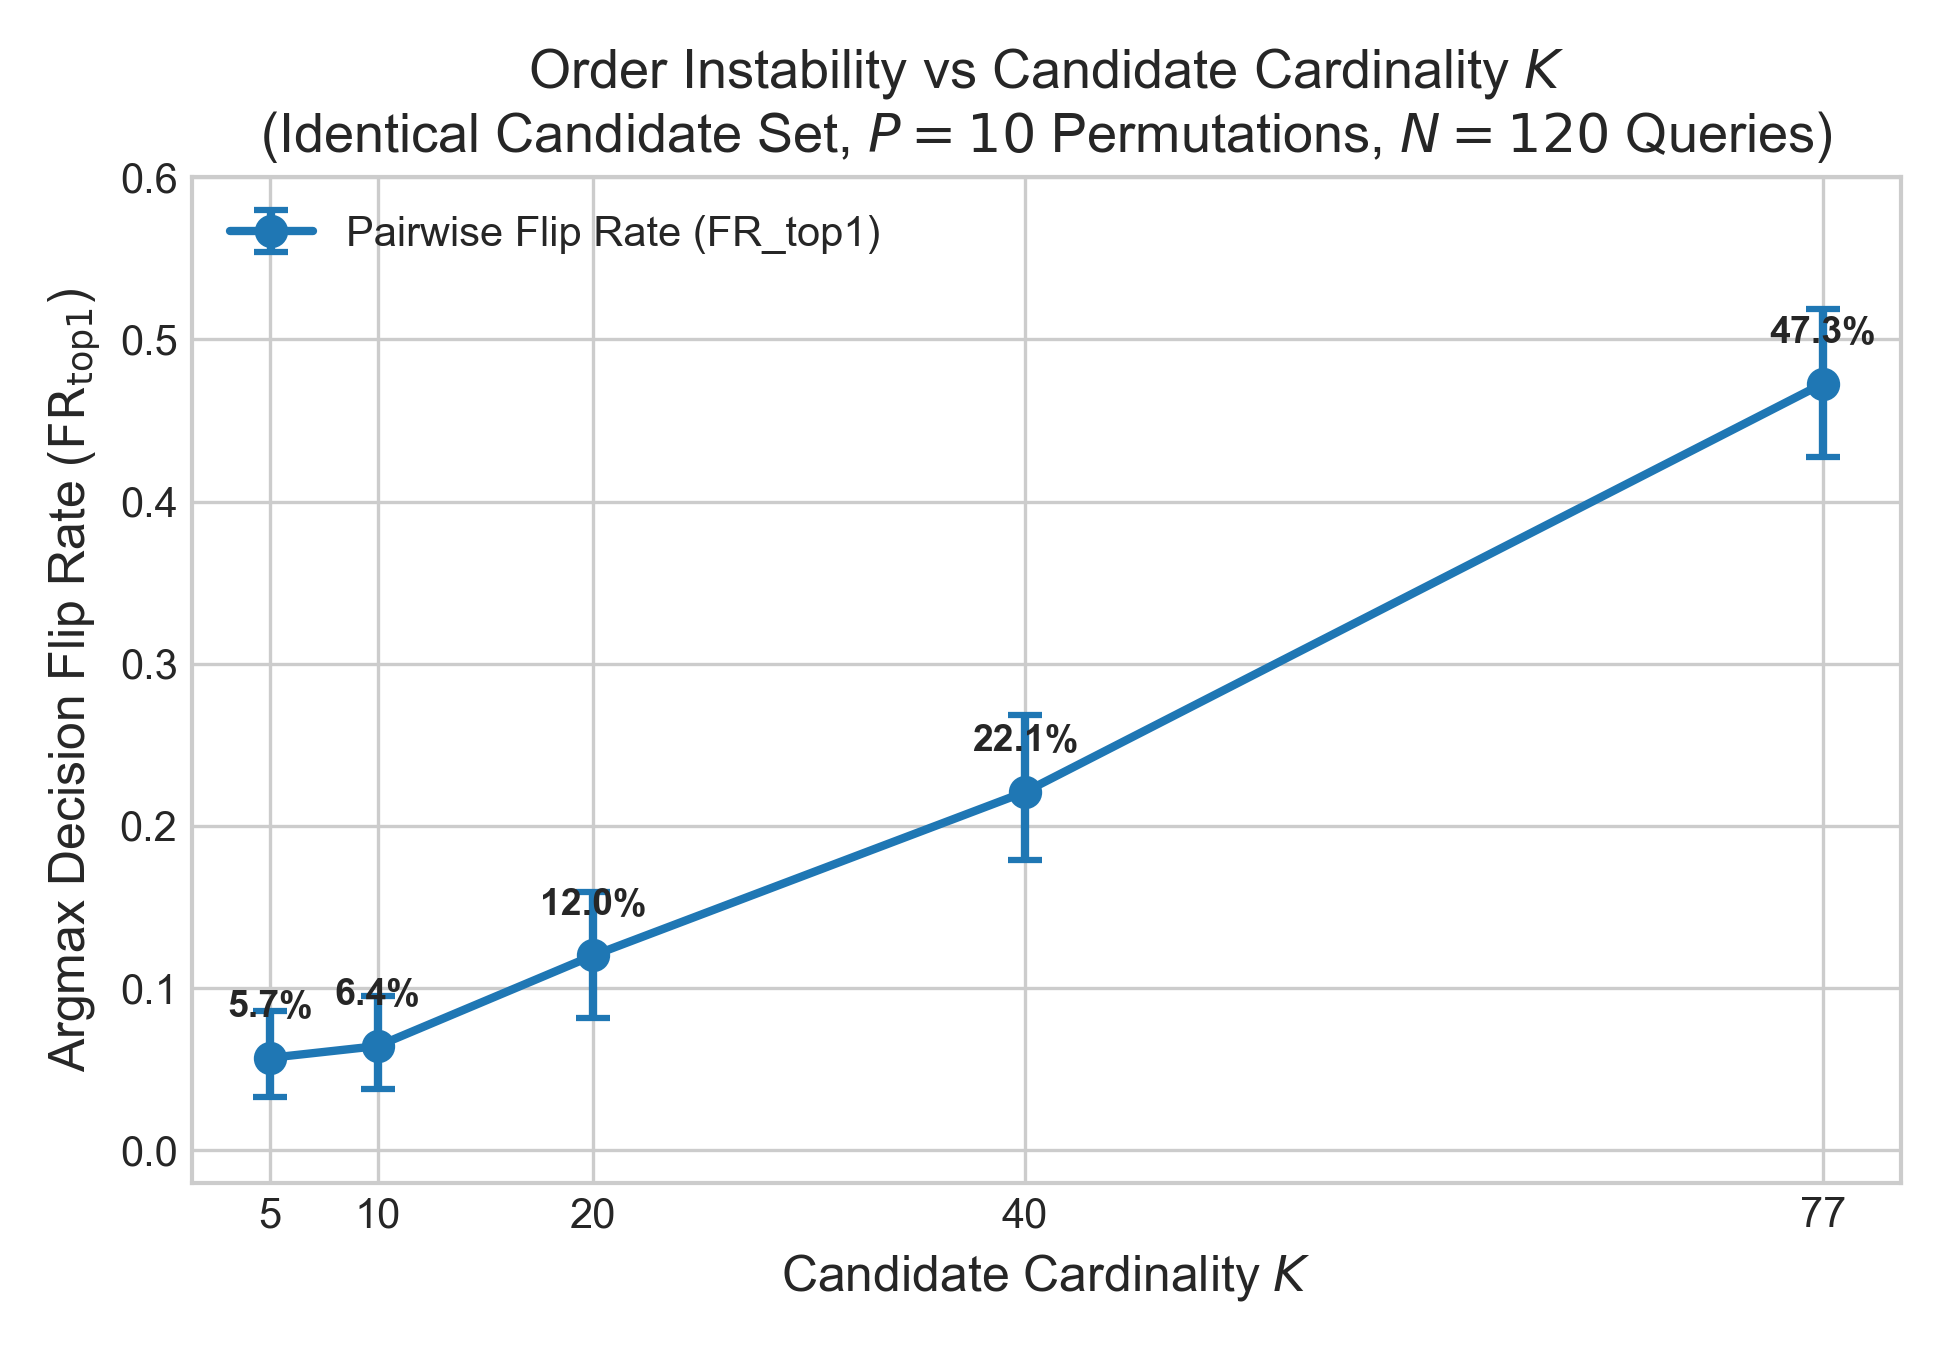
\includegraphics[width=\textwidth]{figures/fig1_cardinality_vs_instability.png}
    \caption{Argmax decision flip rate ($\mathrm{FR}_{\mathrm{top1}}$) scaling.}
    \label{fig:cardinality_instability}
\end{subfigure}
\hfill
\begin{subfigure}[b]{0.48\textwidth}
    \centering
    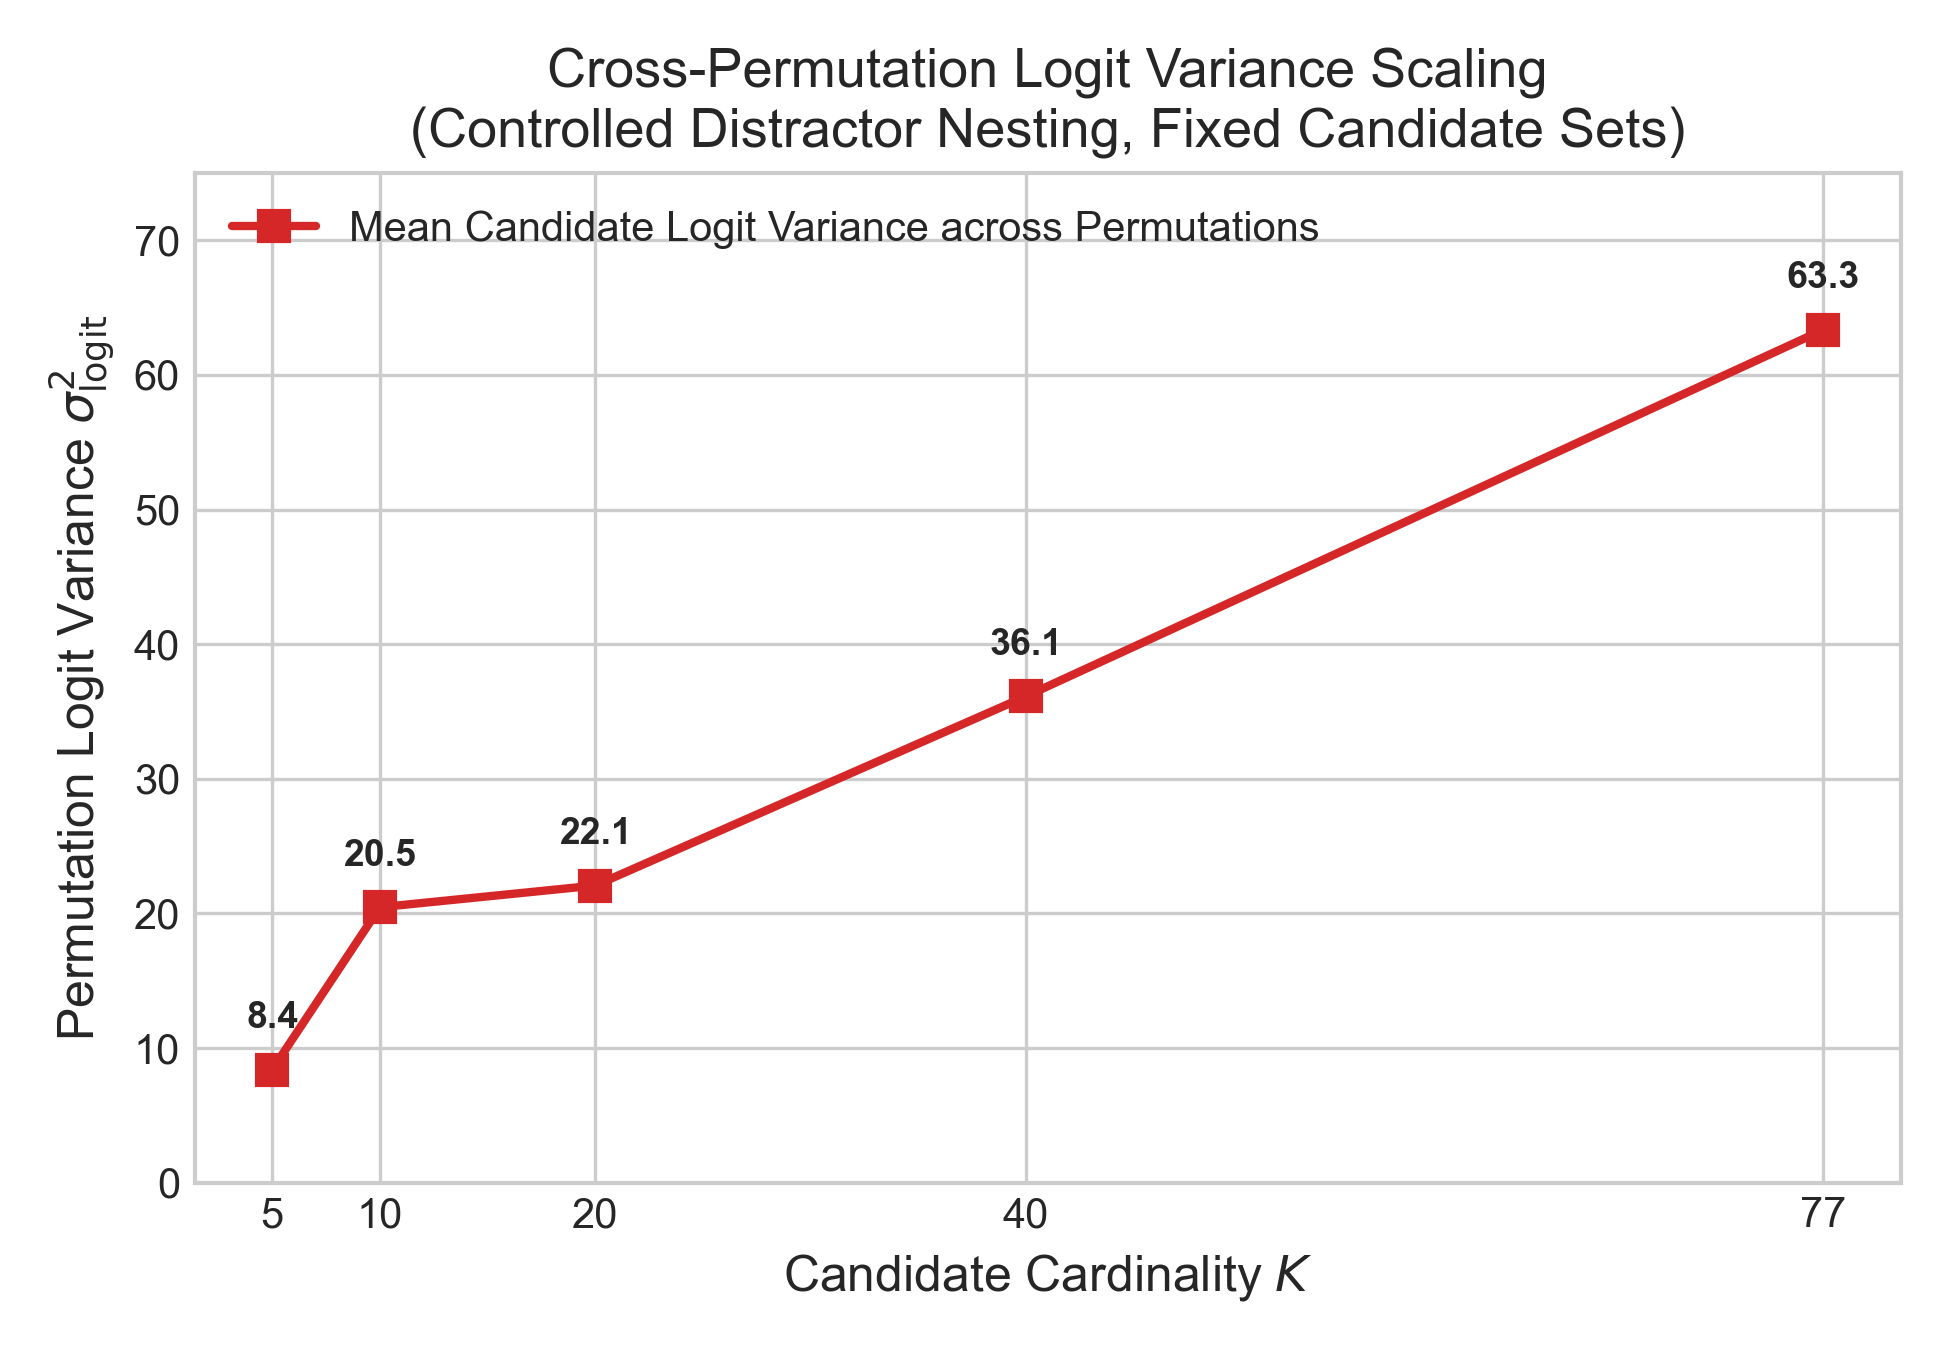
\includegraphics[width=\textwidth]{figures/fig2_cardinality_vs_logit_variance.png}
    \caption{Mean cross-permutation logit variance ($\sigma^2_{\mathrm{logit}}$).}
    \label{fig:logit_variance}
\end{subfigure}
\caption{\textbf{Candidate Cardinality Scaling.} (a) Pairwise decision flip rate $\mathrm{FR}_{\mathrm{top1}}$ strongly increases as candidate cardinality $K$ expands. (b) Mean candidate logit variance across permutations expands by $7.5\times$ ($8.40 \to 63.34$), driven by sequence-length attentional dilution.}
\label{fig:cardinality_scaling}
\end{figure}

This instability is accompanied by a severe expansion in cross-permutation logit volatility. As shown in Figure~\ref{fig:logit_variance}, the mean variance of candidate log-probabilities across permutations increases by $7.5\times$, scaling from $8.40$ at $K=5$ to $63.34$ at $K=77$. As sequence length expands from 60 tokens to over 450 tokens, self-attention entropy distributes over a wider context, increasing marker hidden state variance.

\subsection{The Canonical Ordering Counterfactual}

A common engineering approach to non-deterministic serialization is canonicalization (e.g., sorting candidates alphabetically by label string). Under repeated execution, `B1\_Alpha' achieves perfect repeatability ($\mathrm{FR}_{\mathrm{top1}} \equiv 0.0\%$), giving the illusion of invariance.

\begin{figure}[H]
\centering
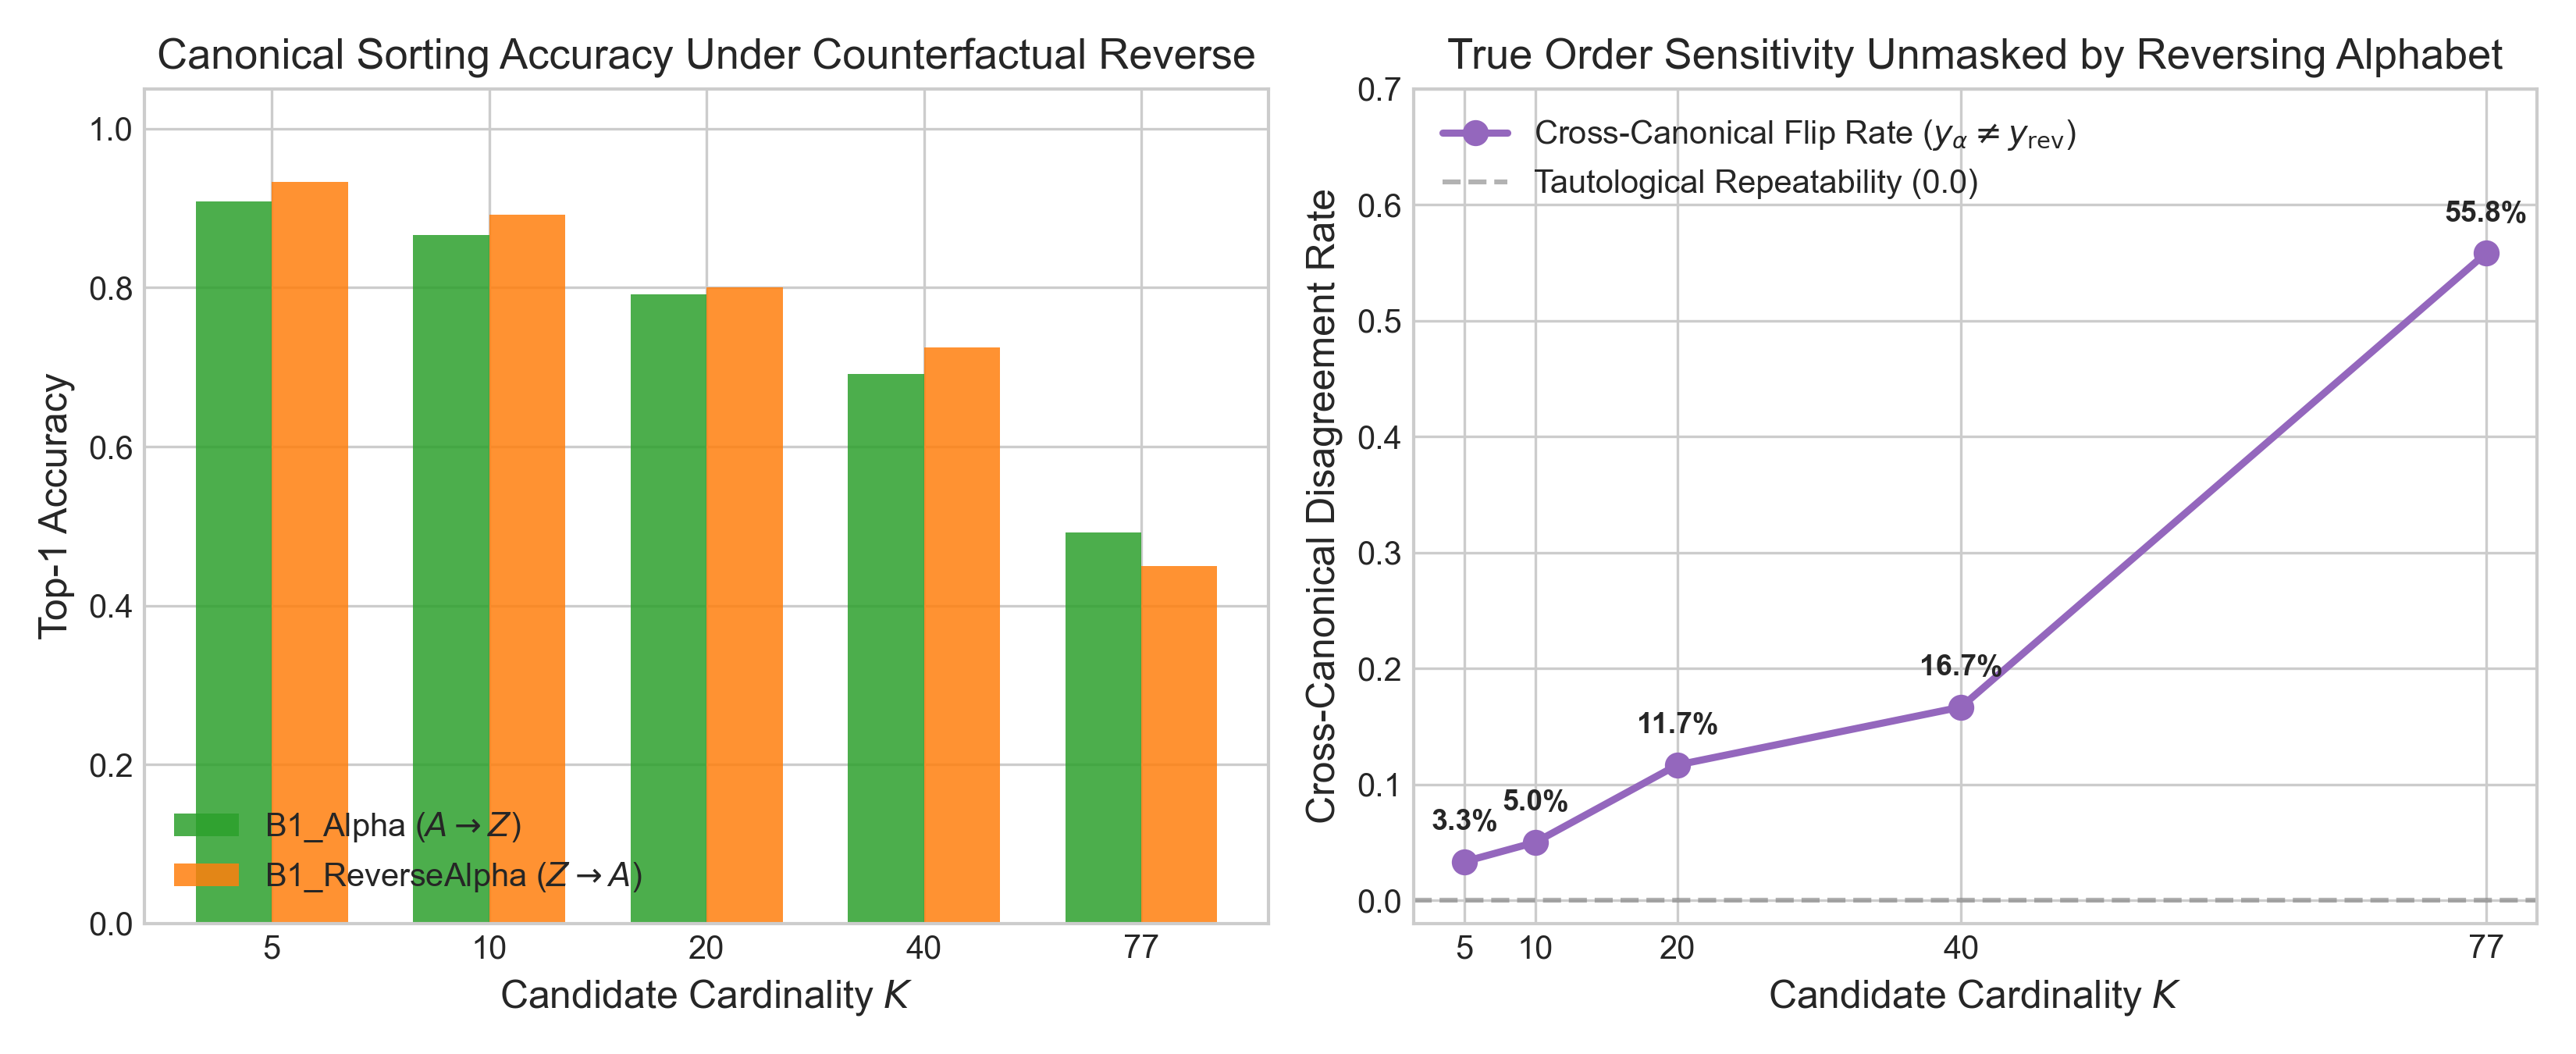
\includegraphics[width=0.88\textwidth]{figures/fig3_canonical_counterfactual.png}
\caption{\textbf{Canonical Counterfactual Analysis.} (Left) Classification accuracy under alphabetical ($A \to Z$) versus reverse alphabetical ($Z \to A$) candidate sorting across cardinalities. (Right) Cross-canonical disagreement rate reaches $55.83\%$ at $K=77$, demonstrating that canonical sorting conceals rather than eliminates underlying positional exposure bias.}
\label{fig:canonical_counterfactual}
\end{figure}

To test whether alphabetical sorting resolves true positional sensitivity, we evaluate the counterfactual reverse-alphabetical ordering (`B1\_ReverseAlpha', $Z \to A$). As depicted in Figure~\ref{fig:canonical_counterfactual}, the cross-canonical flip rate increases from $3.33\%$ [0.8\%, 6.7\%] at $K=5$ to $55.83\%$ [47.5\%, 65.0\%] at $K=77$. At $K=77$, in more than half of all queries, reversing candidate string order alters the model's top-1 classification. Canonicalization does not restore permutation invariance; it merely locks the decision boundary into a static positional bias that systematically favors early-alphabet tokens.

\subsection{Random Marginalization Scaling}

Averaging softmax output probabilities over $M \in \{1, 2, 3, 5\}$ random permutations monotonically reduces residual decision instability. At $K=77$, residual flip rate decreases from $47.28\%$ at $M=1$ down to $38.06\%$ ($M=2$), $34.72\%$ ($M=3$), and $25.83\%$ [20.3\%, 32.0\%] at $M=5$ (Figure~\ref{fig:marginalization_scaling}).

\begin{figure}[H]
\centering
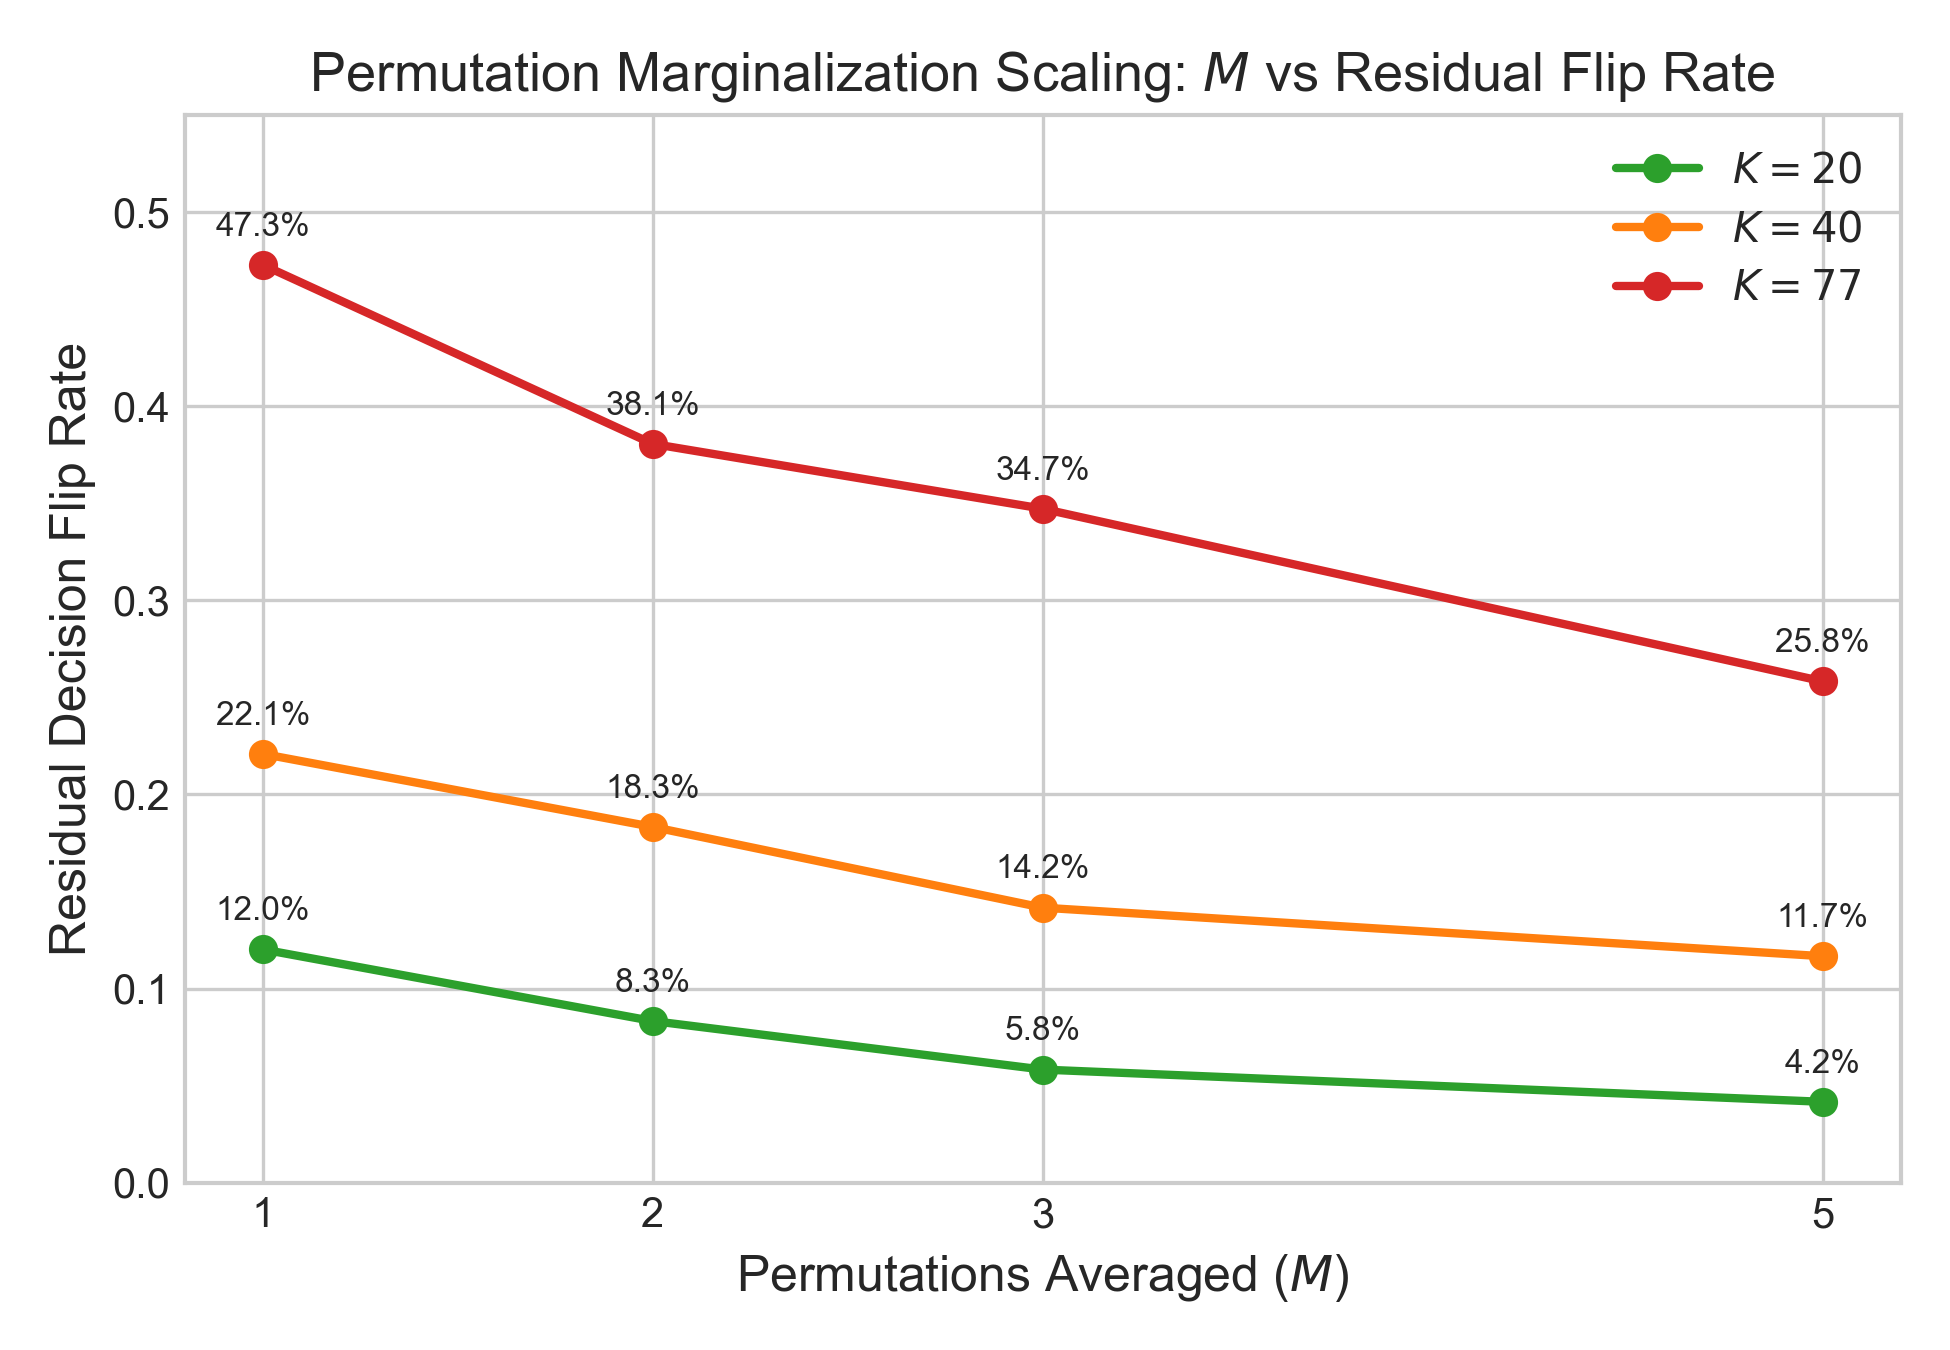
\includegraphics[width=0.65\textwidth]{figures/fig4_marginalization_scaling.png}
\caption{\textbf{Permutation Marginalization Scaling.} Residual decision flip rate decreases monotonically as ensemble passes $M$ increase from 1 to 5 across $K \in \{20, 40, 77\}$.}
\label{fig:marginalization_scaling}
\end{figure}

\subsection{Orthogonal Cyclic Shifts vs.\ Random Marginalization}

Deterministic cyclic permutation shifts (`B2\_Cyclic') distribute candidate markers evenly across all sequence positions using orthogonal phase offsets. At equal computational cost ($M=5$ forward passes), cyclic marginalization achieves a residual flip rate of $16.11\%$ [11.9\%, 20.6\%] at $K=77$, compared to $25.83\%$ [20.3\%, 32.0\%] for random marginalization (Figure~\ref{fig:cyclic_vs_random}). Cyclic shifts provide more uniform positional coverage per forward pass than random uniform sampling.

\begin{figure}[H]
\centering

\includegraphics[width=0.88\textwidth]{figures/fig6_cyclic_vs_random.png}
\caption{\textbf{Cyclic versus Random Marginalization at $K=77$.} (Left) Top-1 accuracy comparison across ensemble budgets $M \in \{2, 3, 5\}$. (Right) Residual decision flip rate: cyclic shifts suppress residual instability to $16.11\%$ at $M=5$, compared to $25.83\%$ for random marginalization.}
\label{fig:cyclic_vs_random}
\end{figure}

\subsection{Probability Calibration and ECE}

As candidate cardinality expands, single-pass models exhibit severe miscalibration: Expected Calibration Error at $K=77$ reaches $0.3700$ [0.30, 0.45] for `B0\_Native' and $0.3857$ [0.31, 0.47] for `B0\_Random'. Inference-time marginalization provides substantial calibration benefits: at $K=77$, `Rand\_Marg\_M5' reduces ECE to $0.0960$ [0.09, 0.20], and `B2\_Cyclic\_M5' reduces ECE to $0.1619$ [0.13, 0.26]. Averaging probability vectors across permutations dampens extreme, overconfident probability spikes.

\subsection{Query-Level Instability Heterogeneity}

Order instability is not distributed uniformly across queries. As illustrated in Figure~\ref{fig:query_heterogeneity}, $55.0\%$ of queries at $K=77$ experience an argmax flip rate $\mathrm{FR}_{\mathrm{top1}} \ge 50\%$, while a minority of queries remain stable. Query instability exhibits a strong negative Pearson correlation with model confidence:
\begin{equation}
r = -0.4926 \quad (p = 1.09 \times 10^{-8}).
\end{equation}
Queries with high predictive margin between the top-1 and top-2 candidates are resilient to serialization perturbations, whereas queries near decision boundaries fluctuate extensively under sequence reordering.

\begin{figure}[H]
\centering
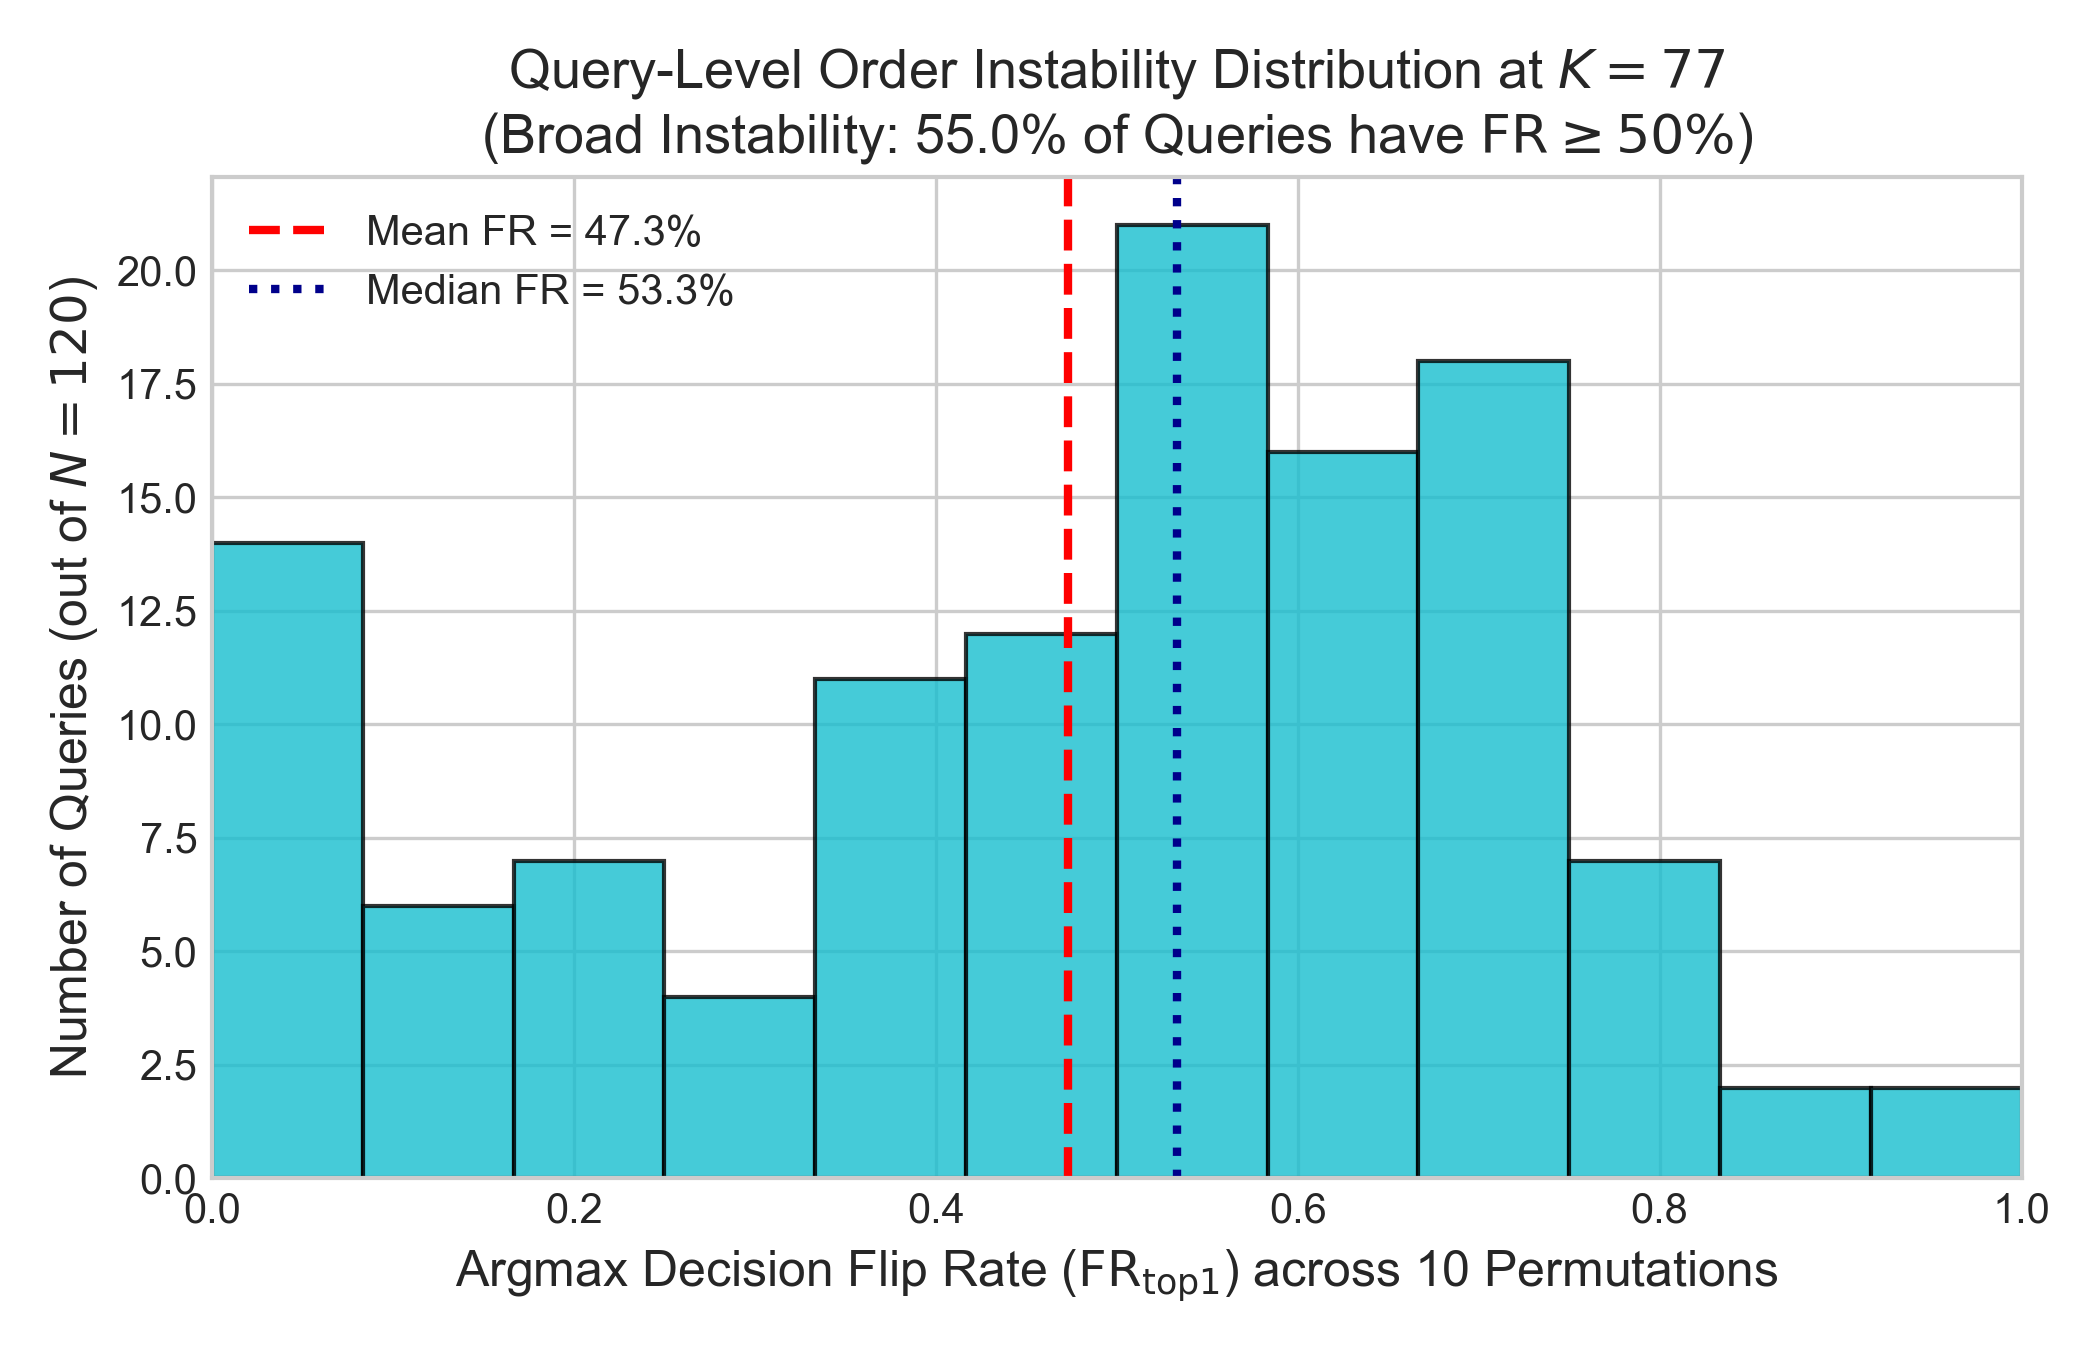
\includegraphics[width=0.68\textwidth]{figures/fig7_k77_query_heterogeneity.png}
\caption{\textbf{Query-Level Instability Distribution at $K=77$.} Distribution of per-query argmax flip rate across 10 random permutations. Over $55.0\%$ of queries experience $\mathrm{FR} \ge 50\%$. Instability is strongly negatively correlated with prediction confidence ($r = -0.4926, p = 1.09 \times 10^{-8}$).}
\label{fig:query_heterogeneity}
\end{figure}

\subsection{Three-Objective Pareto Frontier at \texorpdfstring{$K=77$}{K=77}}

Figure~\ref{fig:pareto_frontier} illustrates the operational trade-offs across Accuracy ($\uparrow$), p50 Latency ($\downarrow$), and within-method Instability ($\downarrow$, measured by $\mathrm{FR}_{\mathrm{top1}}$).

\begin{figure}[H]
\centering
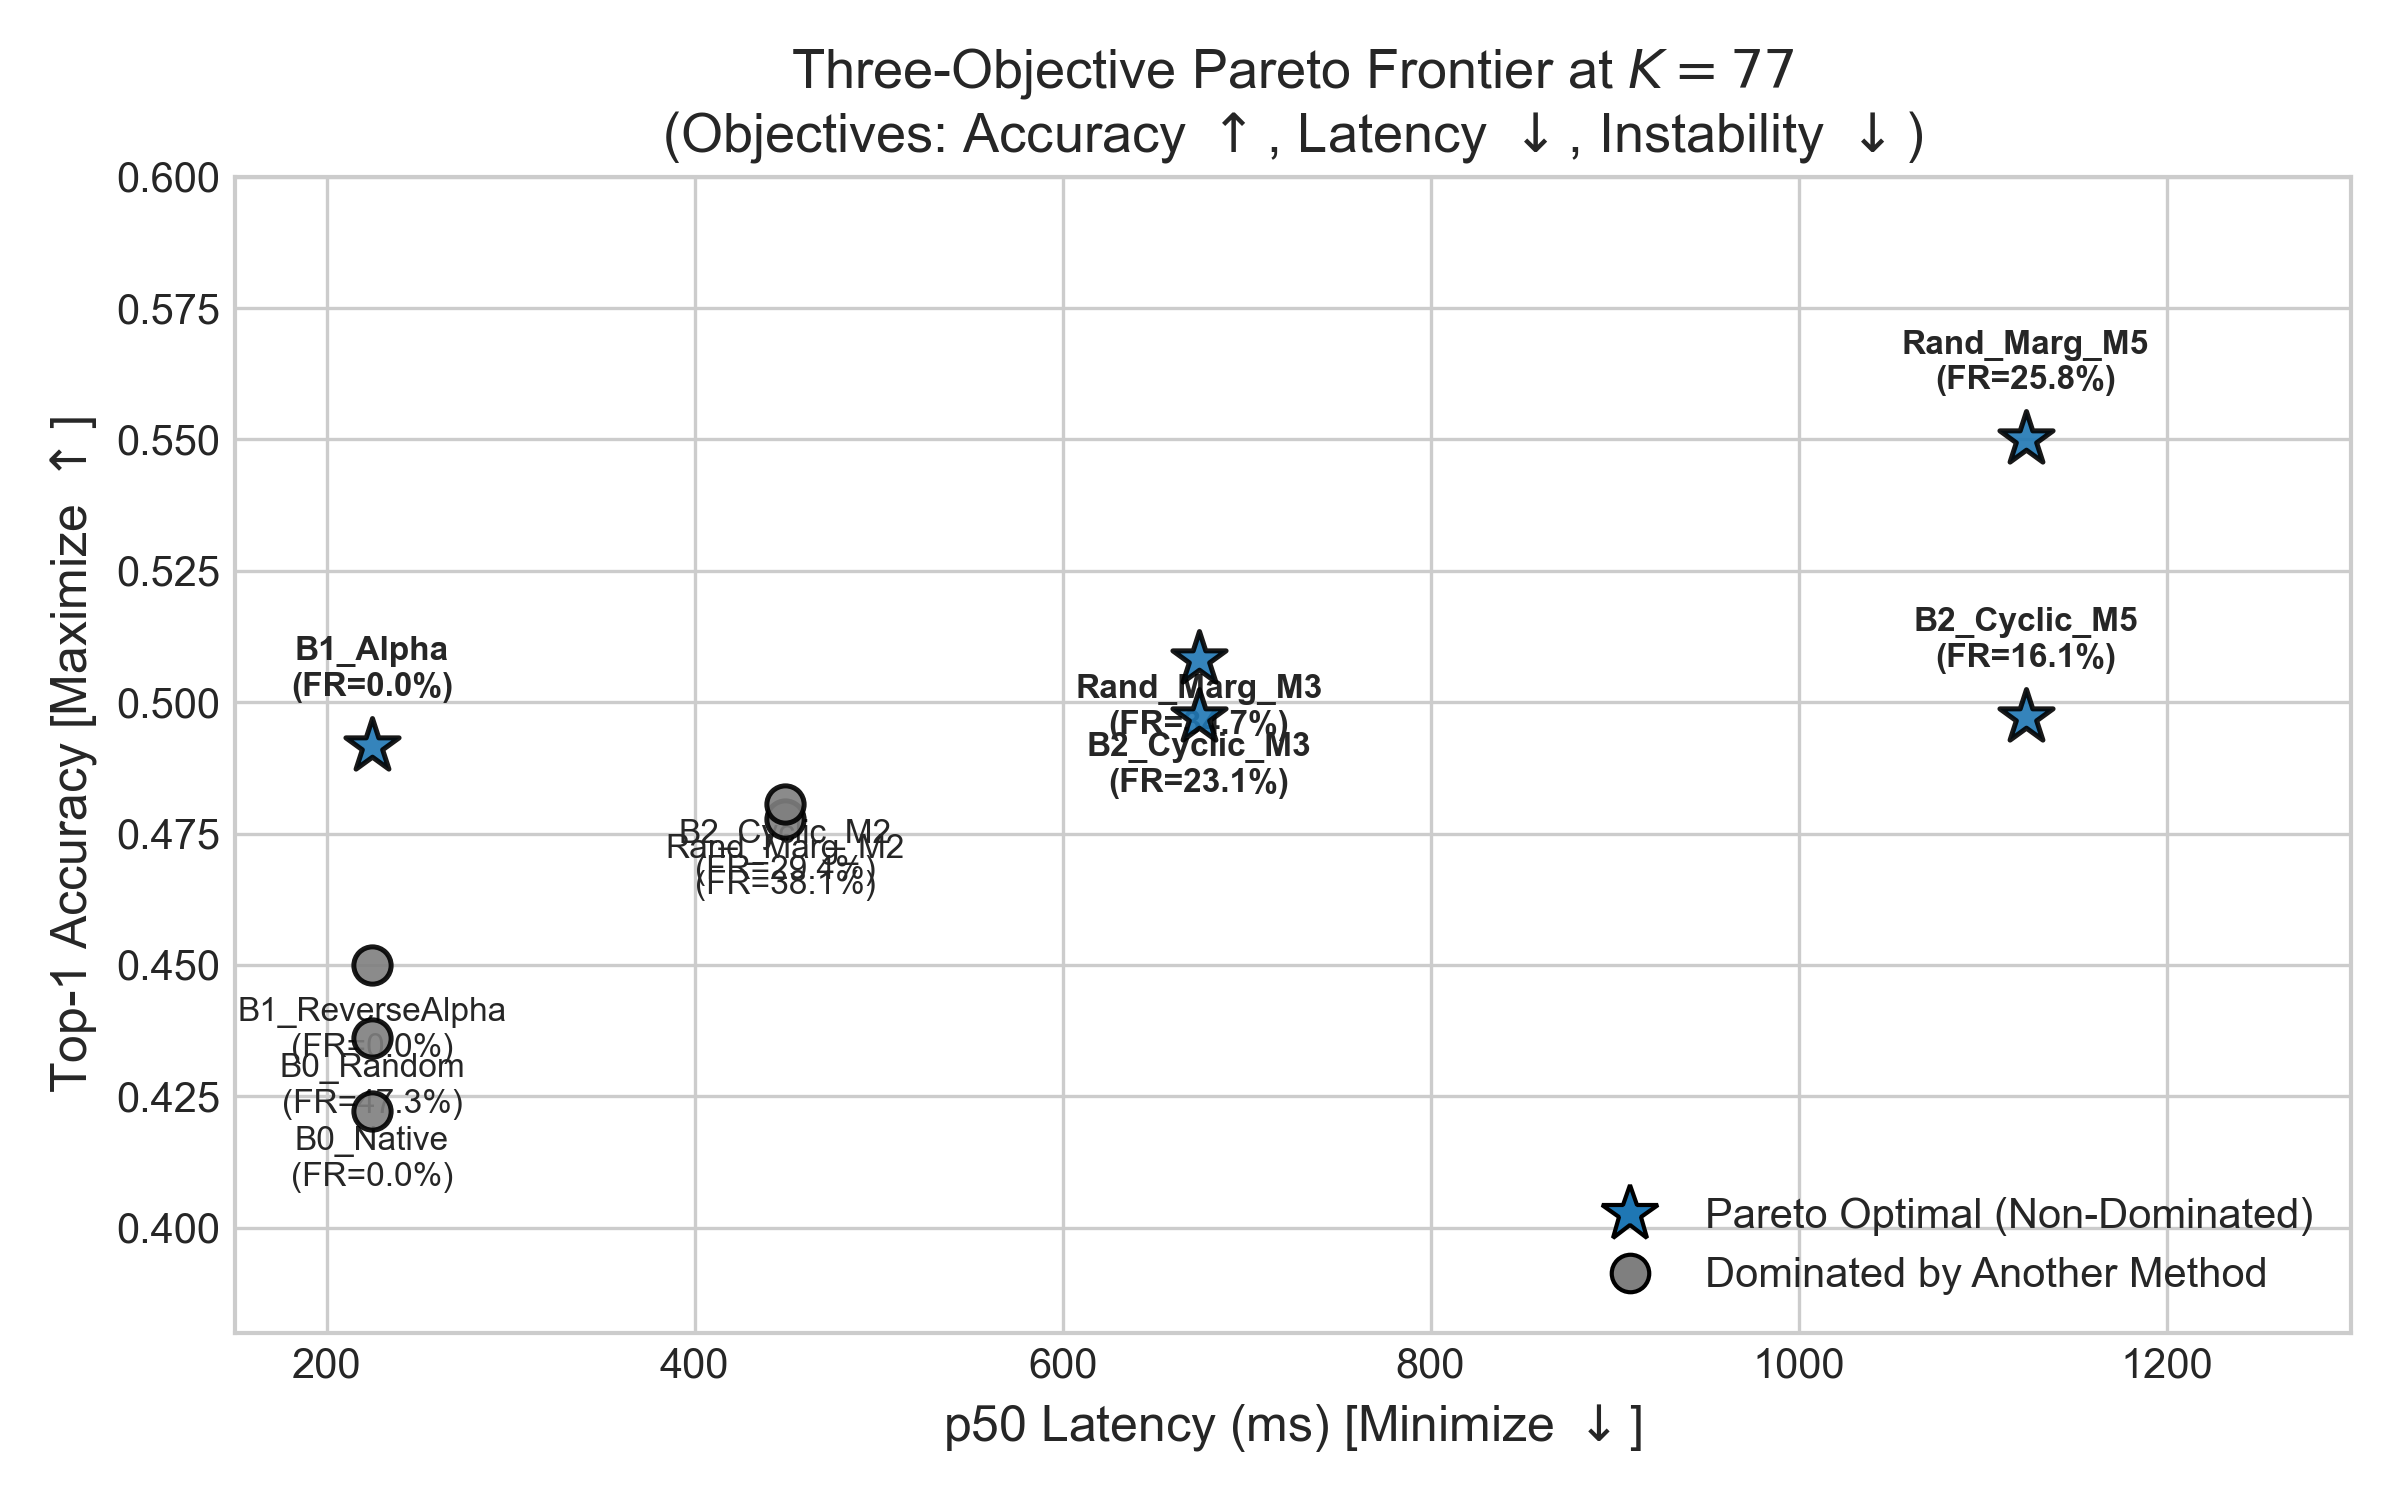
\includegraphics[width=0.75\textwidth]{figures/fig5_pareto_frontier_k77.png}
\caption{\textbf{Three-Objective Pareto Frontier at $K=77$.} Evaluating Accuracy ($\uparrow$), Latency ($\downarrow$), and within-method Instability ($\downarrow$, $\mathrm{FR}_{\mathrm{top1}}$). Non-dominated methods represent Pareto-efficient operating points: `B1\_Alpha' minimizes latency with $0\%$ rerun variance (at the cost of $55.8\%$ cross-canonical exposure bias); `Rand\_Marg\_M5' achieves highest accuracy ($55.0\%$); `B2\_Cyclic\_M5' minimizes residual flip rate ($16.1\%$) among multi-pass methods.}
\label{fig:pareto_frontier}
\end{figure}

\begin{table}[H]
\centering
\small
\caption{\textbf{Detailed Results at Maximum Cardinality ($K=77$).} Evaluated across $N=120$ queries and three base orderings. $\mathrm{FR}_{\mathrm{top1}}$ measures within-method rerun volatility; $\text{Cross-Flip}$ measures counterfactual $A \to Z$ vs $Z \to A$ disagreement.}
\label{tab:k77_detailed}
\resizebox{\columnwidth}{!}{%
\begin{tabular}{l c c c c r c}
\toprule
Method & Accuracy [95\% CI] & ECE [95\% CI] & $\text{FR}_{\text{top1}}$ & Cross-Flip & Latency & Pareto Status \\
\midrule
\textbf{B0\_Native}       & 0.422 [0.34, 0.50] & 0.370 [0.30, 0.45] & 0.000 & --    & 224.7 ms & Dominated \\
\textbf{B0\_Random}       & 0.436 [0.36, 0.51] & 0.386 [0.31, 0.47] & 0.473 & --    & 224.7 ms & Dominated \\
\textbf{B1\_Alpha}        & 0.492 [0.40, 0.58] & 0.334 [0.27, 0.43] & 0.000 & 0.558 & 224.7 ms & \textbf{Non-dominated} \\
\textbf{B1\_ReverseAlpha} & 0.450 [0.37, 0.53] & 0.370 [0.30, 0.46] & 0.000 & 0.558 & 224.7 ms & Dominated \\
\textbf{Rand\_Marg\_M2}   & 0.478 [0.40, 0.55] & 0.202 [0.16, 0.31] & 0.381 & --    & 449.4 ms & Dominated \\
\textbf{Rand\_Marg\_M3}   & 0.508 [0.43, 0.59] & 0.204 [0.16, 0.29] & 0.347 & --    & 674.0 ms & \textbf{Non-dominated} \\
\textbf{Rand\_Marg\_M5}   & \textbf{0.550 [0.47, 0.62]} & \textbf{0.096 [0.09, 0.20]} & 0.258 & -- & 1123.4 ms & \textbf{Non-dominated} \\
\textbf{B2\_Cyclic\_M2}   & 0.481 [0.41, 0.56] & 0.218 [0.16, 0.31] & 0.294 & --    & 449.4 ms & Dominated \\
\textbf{B2\_Cyclic\_M3}   & 0.497 [0.42, 0.57] & 0.147 [0.11, 0.24] & 0.231 & --    & 674.0 ms & \textbf{Non-dominated} \\
\textbf{B2\_Cyclic\_M5}   & 0.497 [0.42, 0.58] & 0.162 [0.13, 0.26] & \textbf{0.161} & -- & 1123.4 ms & \textbf{Non-dominated} \\
\bottomrule
\end{tabular}%
}
\end{table}

\section{Statistical Significance and Hypothesis Testing}

Across all 45 pre-specified paired comparisons against `B0\_Native' under Benjamini-Hochberg False Discovery Rate control ($q=0.05$), exactly \textbf{one comparison achieved statistical significance}:
\begin{itemize}
    \item \textbf{`B2\_Cyclic\_M5' at $K=40$:} Achieved $70.83\%$ accuracy versus $61.67\%$ for `B0\_Native' ($+9.17$ percentage points, 11 discordant gains, 0 losses, unadjusted two-sided exact McNemar $p = 0.0009765625$, BH-adjusted $p = 0.04395$).
\end{itemize}

At $K=77$, although `Rand\_Marg\_M5' observed an apparent accuracy gain of $+12.78$ percentage points ($55.00\%$ vs $42.22\%$, 27 gains, 11 losses, unadjusted $p=0.0145$), this difference \textbf{failed FDR-adjusted statistical significance} (BH-adjusted $p=1.0000$). With $N=120$ queries and binary outcomes, query-level variance precludes declaring $K=77$ accuracy gains statistically significant under rigorous multiple-testing control.

\begin{table}[H]
\centering
\small
\caption{\textbf{Paired Hypothesis Tests vs B0\_Native (Selected Comparisons).} Two-sided exact McNemar tests on discordant classification pairs with Benjamini-Hochberg FDR adjustments ($q=0.05$).}
\label{tab:significance_summary}
\begin{tabular}{r l r c c c c}
\toprule
$K$ & Method & $\Delta$ Accuracy & Gains / Losses & Unadjusted $p$ & BH-Adjusted $p$ & FDR Sig \\
\midrule
5  & B1\_Alpha     & $-1.67\%$ & 1 / 3  & 0.6250   & 1.0000 & No \\
5  & Rand\_Marg\_M5 & $0.00\%$  & 3 / 3  & 1.0000   & 1.0000 & No \\
10 & Rand\_Marg\_M5 & $+0.83\%$ & 1 / 0  & 1.0000   & 1.0000 & No \\
20 & Rand\_Marg\_M5 & $+5.00\%$ & 8 / 2  & 0.1094   & 0.4922 & No \\
40 & B1\_Alpha     & $+7.50\%$ & 10 / 1 & 0.0117   & 0.4922 & No \\
40 & Rand\_Marg\_M5 & $+8.33\%$ & 12 / 2 & 0.0129   & 0.2344 & No \\
\textbf{40} & \textbf{B2\_Cyclic\_M5} & $\mathbf{+9.17\%}$ & \textbf{11 / 0} & $\mathbf{0.00098}$ & $\mathbf{0.04395}$ & \textbf{Yes} ($*$) \\
77 & B1\_Alpha     & $+6.94\%$ & 20 / 12 & 0.2153   & 1.0000 & No \\
77 & B2\_Cyclic\_M5 & $+7.50\%$ & 22 / 13 & 0.1755   & 1.0000 & No \\
77 & Rand\_Marg\_M5 & $+12.78\%$ & 27 / 11 & 0.0145   & 1.0000 & No \\
\bottomrule
\end{tabular}
\end{table}

\section{Important Negative Replication Result}

In preliminary exploratory benchmarking ($N=40, S=1$ base sequence), an anomalous accuracy of \textbf{$65.0\%$} was observed for cyclic shifts ($M=2$) at $K=77$, leading to an initial conjecture that cyclic shifts dramatically improve classification accuracy at full cardinality.

Under our pre-specified replication protocol ($N=120$ unique queries, stratified sampling, $S=3$ independently seeded base candidate sequences `[alphabetical, 7701, 7702]'):
\begin{itemize}
    \item Replicated `B2\_Cyclic\_M2' accuracy is \textbf{$48.06\%$ [39.7\%, 55.6\%]}, statistically indistinguishable from random marginalization ($47.78\%$).
    \item Replicated `B2\_Cyclic\_M5' accuracy is \textbf{$49.72\%$ [41.7\%, 57.2\%]}.
\end{itemize}
This negative result is documented as an integral empirical finding. At high candidate cardinality ($K=77$), small sample sizes ($N=40$) combined with anchoring to a single arbitrary base candidate sequence produce false-positive accuracy spikes. Controlled multi-seed replication corrected this exploratory artifact.

\section{Discussion}

\paragraph{Architecture-Induced Order Sensitivity.}
In contrast to bi-encoders that score candidates independently, multi-candidate concatenation introduces cross-candidate attentional competition. Because token representations are coupled through bidirectional self-attention and positional embeddings, candidate order acts as a hidden nuisance parameter.

\paragraph{Canonicalization vs.\ Permutation Invariance.}
Alphabetical canonicalization is widely used to enforce deterministic model outputs in production pipelines. Our counterfactual analysis demonstrates that canonicalization merely fixes a single arbitrary permutation, concealing underlying order sensitivity. If label strings are translated, renamed, or prefixed, decisions flip on $55.83\%$ of queries at $K=77$.

\paragraph{Inference-Time Marginalization.}
Permutation marginalization provides an inference-time solution without requiring architectural retraining. At $M=5$, orthogonal cyclic shifts reduce residual decision flip rate to $16.11\%$ while reducing Expected Calibration Error from $0.3857$ to $0.1619$. However, marginalization incurs an $M\times$ latency overhead, establishing a clear trade-off between latency and decision stability.

\section{Limitations}

\begin{enumerate}
    \item \textbf{Single Backbone and Checkpoint:} Evaluations were conducted on \texttt{convaiinnovations/\allowbreak laya} (RoBERTa-based bidirectional encoder). While the marker concatenation pattern is general, the exact magnitude of instability may vary across backbones and pretraining objectives.
    \item \textbf{Domain Specialization:} Our study evaluates the Banking77 benchmark. Intent classification provides clean distractor subsets, but semantic dynamics in open-domain tool routing may differ.
    \item \textbf{Inference-Time Scope:} We investigate post-training inference-time interventions; we do not evaluate training-time data augmentation (e.g., training with randomized permutations) or permutation-invariant pooling layers.
    \item \textbf{Statistical Power at $K=77$ ($N=120$):} Detecting a $+5\%$ to $+10\%$ accuracy gain under Benjamini-Hochberg FDR control across 45 comparisons requires $N \ge 350$ queries due to binary classification variance.
\end{enumerate}

\section{Conclusion}

Candidate presentation order induces substantial decision instability in non-autoregressive multi-candidate transformers, scaling from $5.70\%$ at $K=5$ to $47.28\%$ at $K=77$. Canonical alphabetical sorting achieves deterministic repeatability but conceals a $55.83\%$ counterfactual cross-order disagreement rate. Inference-time permutation marginalization systematically suppresses residual instability and improves calibration, with orthogonal cyclic shifts achieving $16.11\%$ residual flip rate at $M=5$. Across 45 pre-specified paired comparisons, cyclic marginalization at $K=40$ achieves the sole statistically significant accuracy improvement ($+9.17$ percentage points, adjusted $p=0.04395$). These findings demonstrate that candidate serialization is an active source of variance in multi-candidate encoders that requires explicit algorithmic marginalization or invariant pooling.

\section*{Reproducibility and Artifact Availability}

To support complete scientific reproducibility, all experimental artifacts, raw evaluations, statistical suites, and figure rendering scripts are permanently archived \citep{saxena2026candidate}:
\begin{itemize}
    \item \textbf{GitHub Repository:} \url{https://github.com/anshull-saxena/candidate-order-instability}
    \item \textbf{Permanent Zenodo DOI:} \href{https://doi.org/10.5281/zenodo.22906245}{10.5281/zenodo.22906245}
    \item \textbf{Archival Release:} \texttt{v1.0.0}
    \item \textbf{Exact Git Commit:} \texttt{266bbb902871dc9974cbf516adea013e3c4eb084}
\end{itemize}

\bibliographystyle{plainnat}
\bibliography{references}

\end{document}
